\documentclass[10pt, aspectratio=169, handout]{beamer}
\usefonttheme{professionalfonts}

\mode<presentation>
{
  \usetheme{Berkeley}
  \usecolortheme{beaver}
  \usefonttheme{default}
  \setbeamertemplate{navigation symbols}{}
  \setbeamertemplate{caption}[numbered]
} 

\setbeamertemplate{footline}{%
  \leavevmode%
  \hbox{%
    \begin{beamercolorbox}[wd=.85\paperwidth,ht=2.5ex,dp=1ex,left]{author in head/foot}%
      \usebeamerfont{author in head/foot}Maxx Seminario, Electronic Circuits, Spring 2026%
    \end{beamercolorbox}%
    \begin{beamercolorbox}[wd=.15\paperwidth,ht=2.5ex,dp=1ex,right]{date in head/foot}%
      \hspace*{0.5em}\insertframenumber{} / \inserttotalframenumber\hspace*{0.5em}%
    \end{beamercolorbox}%
  }%
  \vskip0pt%
}

\usepackage[english]{babel}
\usepackage[utf8]{inputenc}
\usepackage{tikz}
\usepackage{pgfplots}
\usepackage{array}
\usepackage{makecell}
\usepackage{verbatim}
\usepackage{graphicx}
\usepackage{subcaption}
\usepackage{amsfonts}
\usepackage{amsmath}
\usepackage{bm}
\usepackage{epstopdf}
\usepackage[american]{circuitikz}
\usepackage{caption}
\captionsetup{compatibility=false}
\usepackage[absolute,overlay]{textpos}
\usetikzlibrary{calc}
\usetikzlibrary{pgfplots.fillbetween, backgrounds}
\usetikzlibrary{positioning}
\usetikzlibrary{pgfplots.groupplots}
\usetikzlibrary{plotmarks}
\usetikzlibrary{calc}
\usetikzlibrary{decorations.markings}
\usetikzlibrary{arrows.meta}

\usepgfplotslibrary{groupplots}
\pgfplotsset{compat=newest} 

\usepackage{hyperref}
\hypersetup{
    colorlinks=true,
    linkcolor=blue,
    filecolor=magenta,      
    urlcolor=cyan,
}

% Added by Maxx Seminario 01/06/2026 - for colored icons in itemize labels
\usepackage{wasysym} % for smiles and frowns
\newcommand{\neutralface}{%
  \tikz[baseline=-0.6ex]{
    \draw (0,0) circle (0.9ex);
    \fill (-0.35ex,0.25ex) circle (0.12ex);
    \fill ( 0.35ex,0.25ex) circle (0.12ex);
    \draw (-0.35ex,-0.25ex) -- (0.35ex,-0.25ex);
  }%
}
\newcommand{\baditem}{\textcolor{red!70!black}{\frownie}}
\newcommand{\gooditem}{\textcolor{green!60!black}{\smiley}}
\newcommand{\mehitem}{\textcolor{orange!80!black}{\neutralface}}

\title[ECEN 222]{Complex Numbers Review}
\author{Maxx Seminario}
\institute{University of Nebraska-Lincoln}
\date{Spring 2026}

\begin{document}
\begin{frame}
  \titlepage
\end{frame}

\section{Introduction}

\begin{frame}{Why Complex Numbers in Circuits?}
    
    \begin{columns}[t]
    \column{0.48\textwidth}
        \textbf{The Challenge}:
        \begin{itemize}
            \item AC circuits involve sinusoids
            \item Trigonometry gets messy
            \item Need a better mathematical tool
        \end{itemize}
        
        \vspace{1em}
        \textbf{The Solution}:
        \begin{itemize}
            \item Complex numbers simplify AC analysis
            \item Turn trig into algebra
            \item Enable frequency domain methods
        \end{itemize}
    
    \column{0.48\textwidth}
        \textbf{Key Idea}:
        \begin{itemize}
            \item Represent sinusoids as rotating phasors
            \item Use complex exponentials
            \item Mathematics becomes elegant
        \end{itemize}
        
        \vspace{1em}
        \begin{block}{Goal}
            Build intuition with complex numbers to prepare for frequency domain circuit analysis
        \end{block}
    
    \end{columns}
    
\end{frame}

\section{Complex Number Basics}

\begin{frame}{What is a Complex Number?}
    
    \textbf{Definition}: A complex number $z$ has a real part and an imaginary part
    
    \vspace{1em}
    
    \begin{columns}[t]
    \column{0.48\textwidth}
        \textbf{Rectangular Form}:
        \begin{equation*}
            z = a + jb
        \end{equation*}
        where:
        \begin{itemize}
            \item $a$ = real part, $\text{Re}\{z\}$
            \item $b$ = imaginary part, $\text{Im}\{z\}$
            \item $j = \sqrt{-1}$ 
        \end{itemize}
        
        \vspace{0.5em}
        \textbf{Examples}:
        \begin{itemize}
            \item $7$ (purely real, $b=0$)
            \item $j6$ (purely imaginary, $a=0$)
            \item $3 + j4$
        \end{itemize}
    
    \column{0.48\textwidth}
        \textbf{Complex Plane Visualization}:
        
        \begin{center}
        \begin{tikzpicture}[scale=1.1]
            % Axes
            \draw[->] (-0.5,0) -- (4,0) node[right] {Real};
            \draw[->] (0,-0.5) -- (0,3.5) node[above] {Imaginary};
            
            % Grid
            \draw[dotted, gray!50] (0,0) grid (3.5,3);
            
            % Point
            \draw[->, thick, blue] (0,0) -- (3,2.5) node[midway, above left] {$z$};
            \filldraw[blue] (3,2.5) circle (2pt) node[above right] {$a + jb$};
            
            % Components
            \draw[dashed, red] (3,0) node[below] {$a$} -- (3,2.5);
            \draw[dashed, red] (0,2.5) node[left] {$jb$} -- (3,2.5);
            
        \end{tikzpicture}
        \end{center}
        
    \end{columns}
    
\end{frame}

\begin{frame}{Polar Form of Complex Numbers}
    
    Complex numbers can also be expressed in \textbf{polar form}:
    
    \vspace{1em}
    
    \begin{columns}[t]
    \column{0.48\textwidth}
        \textbf{Polar Representation}:
        \begin{equation*}
            z = r \angle \theta = r e^{j\theta}
        \end{equation*}

        \vspace{-0.4cm}

        \begin{itemize}
            \item $r$ = magnitude (length of vector)
            \item $\theta$ = angle (phase)
        \end{itemize}
          
        Rectangular $\to$ Polar:
        \begin{align*}
            r &= \sqrt{a^2 + b^2} = |z| \\
            \theta &= \arctan(b/a)
        \end{align*}
        
        Polar $\to$ Rectangular:
        \begin{align*}
            a &= r \cos(\theta) \\
            b &= r \sin(\theta)
        \end{align*}
    
    \column{0.48\textwidth}
        \textbf{Polar Visualization}:
        
        \begin{center}
        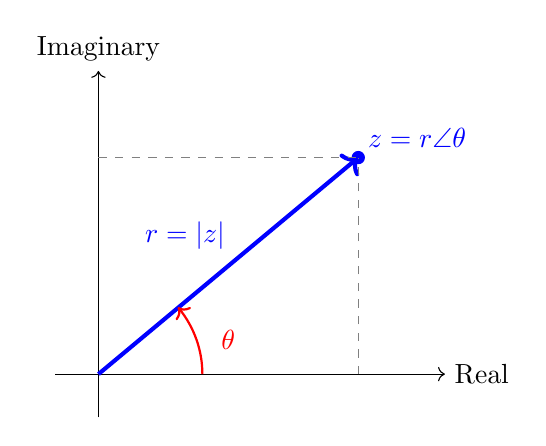
\begin{tikzpicture}[scale=1.1]
            % Axes
            \draw[->] (-0.5,0) -- (4,0) node[right] {Real};
            \draw[->] (0,-0.5) -- (0,3.5) node[above] {Imaginary};
            
            % Point
            \draw[->, thick, blue, line width=1.5pt] (0,0) -- (3,2.5);
            \filldraw[blue] (3,2.5) circle (2pt) node[above right] {$z = r\angle\theta$};
            
            % Magnitude
            \node[blue] at (1.,1.6) {$r = |z|$};
            
            % Angle
            \draw[thick, red, ->] (1.2,0) arc (0:40:1.2);
            \node[red] at (1.5,0.4) {$\theta$};
            
            % Right angle
            \draw[dashed, gray] (3,0) -- (3,2.5);
            \draw[dashed, gray] (0,2.5) -- (3,2.5);
            
        \end{tikzpicture}
        \end{center}
        
    \end{columns}
    
\end{frame}

\section{Euler's Formula and the Unit Circle}

\begin{frame}{Euler's Formula}
    
    \textbf{Euler's Formula} connects complex exponentials to trigonometry:
    
    \begin{equation*}
        \boxed{e^{j\theta} = \cos(\theta) + j\sin(\theta)}
    \end{equation*}
    
    \vspace{1em}
    
    \begin{columns}[t]
    \column{0.48\textwidth}

        \vspace{-0.6cm}

        \textbf{Key Insights}:
        \begin{itemize}
            \item $e^{j\theta}$ represents rotation
            \item Real part: $\cos(\theta)$
            \item Imaginary part: $\sin(\theta)$
            \item Magnitude is always 1
        \end{itemize}
        
        \vspace{-0.7cm}

        \begin{align*}
            e^{j0} &= 1 \\
            e^{j\pi/2} &= j \\
            e^{j\pi} &= -1 \\
            e^{j3\pi/2} &= -j \\
        \end{align*}
    
    \column{0.48\textwidth}
        \textbf{The Unit Circle}:
        
        \begin{center}
        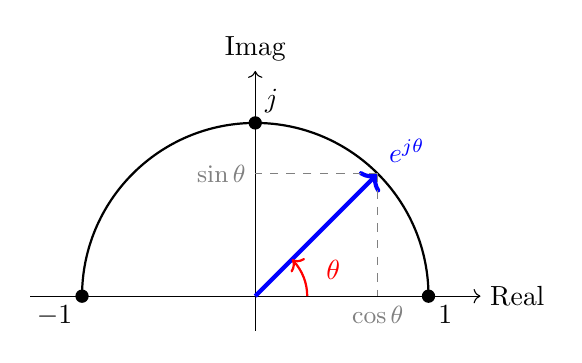
\begin{tikzpicture}[scale=2.2]
            % Top half of circle only
            \draw[thick] (-1,0) arc (180:0:1);
            
            % Axes
            \draw[->] (-1.3,0) -- (1.3,0) node[right] {Real};
            \draw[->] (0,-0.2) -- (0,1.3) node[above] {Imag};
            
            % Key points
            \filldraw (1,0) circle (1pt) node[below right] {$1$};
            \filldraw (0,1) circle (1pt) node[above right] {$j$};
            \filldraw (-1,0) circle (1pt) node[below left] {$-1$};
            
            % Rotating phasor
            \draw[->, thick, blue, line width=1.5pt] (0,0) -- (45:1) node[above right] {$e^{j\theta}$};
            \draw[thick, red, ->] (0.3,0) arc (0:45:0.3);
            \node[red] at (0.45,0.15) {$\theta$};
            
            % Projections
            \draw[dashed, gray] (45:1) -- ({cos(45)},0) node[below] {\small $\cos\theta$};
            \draw[dashed, gray] (45:1) -- (0,{sin(45)}) node[left] {\small $\sin\theta$};
            
        \end{tikzpicture}
        \end{center}
        
    \end{columns}
    
\end{frame}

\begin{frame}{General Polar Form with Euler's Formula}
    
    Any complex number can be written using Euler's formula:
    
    \begin{equation*}
        \boxed{z = r e^{j\theta} = r[\cos(\theta) + j\sin(\theta)] = r\cos(\theta) + jr\sin(\theta)}
    \end{equation*}
    
    \vspace{1em}
    
    \begin{columns}[t]
    \column{0.48\textwidth}
        \textbf{Why This Matters}:
        \begin{itemize}
            \item Multiplication becomes addition of angles
            \item Division becomes subtraction of angles
            \item Powers become angle multiplication
            \item Rotation is just adding to $\theta$
        \end{itemize}
        
        \vspace{0.5em}
        \textbf{Example}: Multiply $2e^{j30°} \times 3e^{j45°}$
        \begin{align*}
            &= (2 \times 3) \cdot e^{j(30° + 45°)} \\
            &= 6 e^{j75°}
        \end{align*}
        
        Much easier than rectangular form!
    
    \column{0.48\textwidth}
        \textbf{Visualizing Rotation}:
        
        \begin{center}
        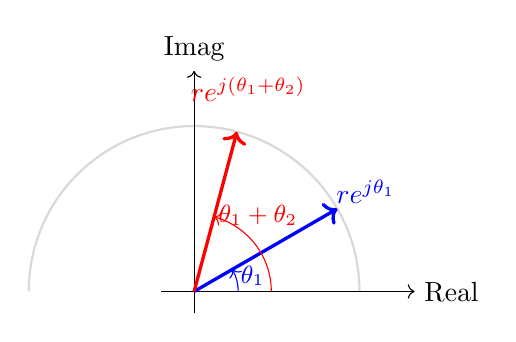
\begin{tikzpicture}[scale=1.4]
            % Top half of circle only
            \draw[thick, gray!30] (-1.5,0) arc (180:0:1.5);
            
            % Axes
            \draw[->] (-0.3,0) -- (2,0) node[right] {Real};
            \draw[->] (0,-0.2) -- (0,2) node[above] {Imag};
            
            % First phasor
            \draw[->, thick, blue, line width=1.2pt] (0,0) -- (30:1.5);
            \node[blue] at (30:1.8) {$re^{j\theta_1}$};
            
            % Second phasor (multiplied)
            \draw[->, thick, red, line width=1.2pt] (0,0) -- (75:1.5);
            \node[red] at (75:1.9) {$re^{j(\theta_1+\theta_2)}$};
            
            % Angle arcs
            \draw[blue, ->] (0.4,0) arc (0:30:0.4);
            \node[blue] at (15:0.55) {\small $\theta_1$};
            
            \draw[red, ->] (0.7,0) arc (0:75:0.7);
            \node[red] at (50:0.9) {\small $\theta_1+\theta_2$};
            
        \end{tikzpicture}
        \end{center}
        
        Multiplying by $e^{j\theta_2}$ rotates by angle $\theta_2$
        
    \end{columns}
    
\end{frame}

\section{Operations with Complex Numbers}

\begin{frame}{Addition and Subtraction}
    
    \textbf{Rule}: Add/subtract complex numbers in \textit{rectangular form}
    
    \begin{columns}[t]
    \column{0.48\textwidth}
        \textbf{Addition}:
        \begin{equation*}
            z_1 + z_2 = (a_1 + jb_1) + (a_2 + jb_2)
        \end{equation*}
        \begin{equation*}
            = (a_1 + a_2) + j(b_1 + b_2)
        \end{equation*}
        
        \vspace{-0.2cm}

        \textbf{Example}:
        \begin{align*}
            &(3 + j4) + (2 - j1) \\
            &= (3+2) + j(4-1) \\
            &= 5 + j3
        \end{align*}
        
        \vspace{-0.2cm}

        \textbf{Geometric Interpretation}:
        \begin{itemize}
            \item Add like vectors
            \item Tip-to-tail method
        \end{itemize}
    
    \column{0.48\textwidth}
        \textbf{Vector Addition Visualization}:
        
        \begin{center}
        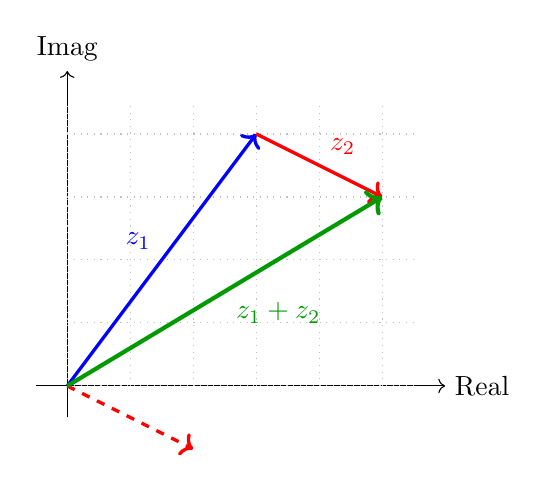
\begin{tikzpicture}[scale=0.8]
            % Axes
            \draw[->] (-0.5,0) -- (6,0) node[right] {Real};
            \draw[->] (0,-0.5) -- (0,5) node[above] {Imag};
            \draw[dotted, gray!50] (0,0) grid (5.5,4.5);
            
            % First vector
            \draw[->, thick, blue, line width=1.2pt] (0,0) -- (3,4) node[midway, above left] {$z_1$};
            
            % Second vector from origin
            \draw[->, thick, red, line width=1.2pt, dashed] (0,0) -- (2,-1);
            
            % Second vector from tip of first
            \draw[->, thick, red, line width=1.2pt] (3,4) -- (5,3) node[midway, above right] {$z_2$};
            
            % Result
            \draw[->, thick, green!60!black, line width=1.5pt] (0,0) -- (5,3) node[midway, below right] {$z_1 + z_2$};
            
        \end{tikzpicture}
        \end{center}
        
    \end{columns}
    
\end{frame}

\begin{frame}{Multiplication and Division}
    
    \textbf{Rule}: Multiply/divide complex numbers in \textit{polar form}
    
    \vspace{1em}
    
    \begin{columns}[t]
    \column{0.48\textwidth}
        \textbf{Multiplication}:
        \begin{equation*}
            z_1 \cdot z_2 = r_1 e^{j\theta_1} \cdot r_2 e^{j\theta_2}
        \end{equation*}
        \begin{equation*}
            = (r_1 r_2) e^{j(\theta_1 + \theta_2)}
        \end{equation*}
        
        \begin{itemize}
            \item Multiply magnitudes: $r_1 \times r_2$
            \item Add angles: $\theta_1 + \theta_2$
        \end{itemize}
        
        \vspace{0.5em}
        \textbf{Example}:
        \begin{align*}
            &(2\angle 30°) \times (3\angle 45°) \\
            &= 6\angle 75°
        \end{align*}
        
    \column{0.48\textwidth}
        \textbf{Division}:
        \begin{equation*}
            \frac{z_1}{z_2} = \frac{r_1 e^{j\theta_1}}{r_2 e^{j\theta_2}}
        \end{equation*}
        \begin{equation*}
            = \frac{r_1}{r_2} e^{j(\theta_1 - \theta_2)}
        \end{equation*}
        
        \begin{itemize}
            \item Divide magnitudes: $r_1 / r_2$
            \item Subtract angles: $\theta_1 - \theta_2$
        \end{itemize}
        
        \vspace{0.5em}
        \textbf{Example}:
        \begin{align*}
            &\frac{10\angle 60°}{2\angle 20°} \\
            &= 5\angle 40°
        \end{align*}
        
    \end{columns}
    
    \vspace{1em}
    
    \begin{alertblock}{Key Point}
        This is why polar form is so powerful! Multiplication/division in rectangular form requires messy algebra.
    \end{alertblock}
    
\end{frame}

\begin{frame}{Complex Conjugate}
    
    The \textbf{complex conjugate} $z^*$ flips the sign of the imaginary part:
    
    \vspace{1em}
    
    \begin{columns}[t]
    \column{0.48\textwidth}
        \textbf{Definitions}:
        
        If $z = a + jb$, then:
        \begin{equation*}
            z^* = a - jb
        \end{equation*}
        
        If $z = r e^{j\theta}$, then:
        \begin{equation*}
            z^* = r e^{-j\theta}
        \end{equation*}

        \textbf{Properties}:
        \begin{itemize}
            \item $z \cdot z^* = |z|^2 = r^2$
            \item $(z^*)^* = z$
            \item $(z_1 + z_2)^* = z_1^* + z_2^*$
            \item $(z_1 \cdot z_2)^* = z_1^* \cdot z_2^*$
        \end{itemize}
    
    \column{0.48\textwidth}
        \textbf{Geometric Visualization}:
        
        \begin{center}
        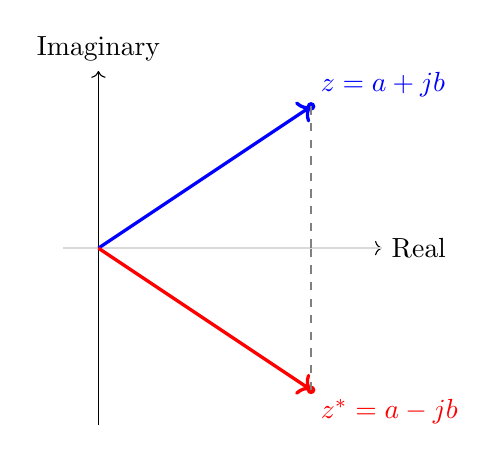
\begin{tikzpicture}[scale=0.9]
            % Axes
            \draw[->] (-0.5,0) -- (4,0) node[right] {Real};
            \draw[->] (0,-2.5) -- (0,2.5) node[above] {Imaginary};
            
            % Real axis
            \draw[thick, gray!30] (-0.5,0) -- (4,0);
            
            % Original number
            \draw[->, thick, blue, line width=1.2pt] (0,0) -- (3,2);
            \filldraw[blue] (3,2) circle (1.5pt) node[above right] {$z = a + jb$};
            
            % Conjugate
            \draw[->, thick, red, line width=1.2pt] (0,0) -- (3,-2);
            \filldraw[red] (3,-2) circle (1.5pt) node[below right] {$z^* = a - jb$};
            
            % Dashed connections
            \draw[dashed, gray] (3,2) -- (3,0);
            \draw[dashed, gray] (3,-2) -- (3,0);
            
        \end{tikzpicture}
        \end{center}
        
        \vspace{0.3em}
        \textbf{Key Use}: Rationalizing denominators
        \begin{equation*}
            \frac{1}{a + jb} = \frac{a - jb}{(a+jb)(a-jb)} = \frac{a - jb}{a^2 + b^2}
        \end{equation*}
        
    \end{columns}
    
\end{frame}

\section{Connection to AC Circuits}

\begin{frame}{Sinusoids and Complex Exponentials}
    
    \textbf{Key Connection}: Sinusoids can be represented as complex exponentials
    
    \vspace{1em}
    
    \begin{columns}[t]
    \column{0.48\textwidth}
        \textbf{From Euler's Formula}:
        \begin{align*}
            e^{j\omega t} &= \cos(\omega t) + j\sin(\omega t) \\
            e^{-j\omega t} &= \cos(\omega t) - j\sin(\omega t) \\
            \cos(\omega t) &= \frac{e^{j\omega t} + e^{-j\omega t}}{2} \\
            \sin(\omega t) &= \frac{e^{j\omega t} - e^{-j\omega t}}{2j}
        \end{align*}
        
        \vspace{-0.3cm}

        \textbf{General Sinusoid}:
        \begin{equation*}
            v(t) = V_m \cos(\omega t + \phi)
        \end{equation*}
        % can be written as:
        \begin{equation*}
            v(t) = \text{Re}\{V_m e^{j(\omega t + \phi)}\}
        \end{equation*}
    
    \column{0.48\textwidth}
        \textbf{Rotating Phasor Interpretation}:
        
        \begin{center}
        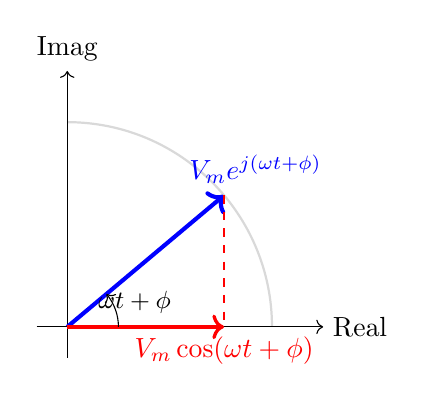
\begin{tikzpicture}[scale=1.3]
            % Top right quadrant of circle only
            \draw[thick, gray!30] (2,0) arc (0:90:2);
            
            % Axes
            \draw[->] (-0.3,0) -- (2.5,0) node[right] {Real};
            \draw[->] (0,-0.3) -- (0,2.5) node[above] {Imag};
            
            % Rotating phasor at angle
            \draw[->, thick, blue, line width=1.5pt] (0,0) -- (40:2);
            \node[blue] at (40:2.4) {$V_m e^{j(\omega t + \phi)}$};
            
            % Projection on real axis
            \draw[dashed, red, thick] (40:2) -- ({2*cos(40)},0);
            \draw[->, thick, red, line width=1.2pt] (0,0) -- ({2*cos(40)},0);
            \node[red, below] at ({2*cos(40)},0) {$V_m\cos(\omega t + \phi)$};
            
            % Angle
            \draw[->] (0.5,0) arc (0:40:0.5);
            \node at (20:0.7) {\small $\omega t + \phi$};
            
        \end{tikzpicture}
        \end{center}
        
        \vspace{-0.3cm}
        The real part of the rotating phasor gives us the sinusoid in the time domain
        
    \end{columns}
    
\end{frame}

\begin{frame}{Phasor Representation}
    
    \textbf{Phasor}: A complex number representing amplitude and phase of a sinusoid
    
    \vspace{1em}
    
    \begin{columns}[t]
    \column{0.48\textwidth}
        \textbf{Time Domain} $\to$ \textbf{Phasor Domain}:
        
        \vspace{-0.2cm}

        \begin{equation*}
            v(t) = V_m \cos(\omega t + \phi)
        \end{equation*}

        \vspace{-0.4cm}

        \begin{equation*}
            \boxed{\mathbf{V} = V_m e^{j\phi} = V_m \angle \phi}
        \end{equation*}
        
        \begin{itemize}
            \item Drop the $e^{j\omega t}$ time dependence
            \item Keep magnitude $V_m$ and phase $\phi$
        \end{itemize}

        \textbf{Examples}:
        \begin{align*}
            10\cos(\omega t + 30°) &\to 10\angle 30° \\
            5\sin(\omega t) &\to 5\angle -90° \\
            -3\cos(\omega t) &\to 3\angle 180°
        \end{align*}
    
    \column{0.48\textwidth}
        \textbf{Why Phasors?}
        \begin{itemize}
            \item[\gooditem] Easy to add sinusoids
            \item[\gooditem] Simplifies circuit analysis
            \item[\gooditem] Natural for AC steady-state
        \end{itemize}
        
        \vspace{-0.1cm}
        \textbf{Adding Sinusoids}:
        
        \begin{itemize}
            \item[\baditem] Time domain (difficult):
                \vspace{-0.2cm}
                \begin{align*}
                    &v_1(t) + v_2(t) = 10\cos(\omega t + 30°) + 5\cos(\omega t - 45°)
                \end{align*}
            \item[\gooditem]  Phasor domain (easy):
             \vspace{-0.2cm}
                \begin{align*}
                    \mathbf{V} &= 10\angle 30° + 5\angle -45° \\
                    &= (8.66 + j5) + (3.54 - j3.54) = 12.2 + j1.46 \\
                    &= 12.3\angle 6.8°
                \end{align*}
        \end{itemize}
        
    \end{columns}
    
\end{frame}

\section{Summary}

\begin{frame}{Summary: Complex Numbers for Circuit Analysis}
    
    \begin{columns}[t]
    \column{0.48\textwidth}
        \textbf{Concepts}:
        \begin{itemize}
            \item Complex numbers: $z = a + jb$
            \item Polar form: $z = r e^{j\theta} = r\angle\theta$
            \item Euler's formula: $e^{j\theta} = \cos\theta + j\sin\theta$
            \item Unit circle representation
        \end{itemize}
        
        \vspace{0.5em}
        \textbf{Operations}:
        \begin{itemize}
            \item Add/subtract in rectangular form
            \item Multiply/divide in polar form
            \item Complex conjugate: $z^* = a - jb$
        \end{itemize}
        
    \column{0.48\textwidth}
        \textbf{For Circuit Analysis}:
        \begin{itemize}
            \item Sinusoids $\leftrightarrow$ Rotating phasors
            \item Time domain $\leftrightarrow$ Frequency domain
            \item Phasors capture magnitude \& phase
            \item Simplify AC circuit analysis
        \end{itemize}
        
        \vspace{0.5em}
        \textbf{Next Lecture}:
        \begin{itemize}
            \item Apply to impedance ($Z$)
            \item Analyze AC circuits with phasors
            \item Frequency domain methods
        \end{itemize}
        
    \end{columns}
    
    \vspace{1em}
    
    \begin{block}{Remember}
        Complex numbers are mathematical tools to make computation easier when dealing with sinusoidal signals in circuits. You will get the same result if you compute in time domain.
    \end{block}
    
\end{frame}

\begin{frame}{Practice Problems}
    
    \textbf{Try these to check your understanding}:
    
    \vspace{1em}
    
    \begin{enumerate}
        \item Convert $4 + j3$ to polar form.
        
        \vspace{0.5em}
        \item Convert $10\angle 135°$ to rectangular form.
        
        \vspace{0.5em}
        \item Compute: $(2 + j3) + (1 - j5)$
        
        \vspace{0.5em}
        \item Compute: $(5\angle 60°) \times (2\angle 30°)$
        
        \vspace{0.5em}
        \item Find the complex conjugate of $3 - j4$.
        
        \vspace{0.5em}
        \item Express $v(t) = 15\cos(\omega t + 45°)$ as a phasor.
        
        \vspace{0.5em}
        \item Add the phasors: $8\angle 0° + 6\angle 90°$
        
    \end{enumerate}
    
\end{frame}

\end{document}
